\subsection{Configuración de \gls{term:grafana}}
\label{configuracion-de-grafana}

Como hemos mencionado anteriormente, hemos elegido \gls{term:grafana} para la
creación de los tableros que mostraran la información que hemos recolectado en
el \autoref{cap3}.

Para iniciar el servicio de \gls{term:grafana} en \gls{term:linux}, basta con
ejecutar el siguiente comando en la terminal:

\begin{lstlisting}
$ sudo service grafana-server start
\end{lstlisting}

Esta orden inicializa el proceso \texttt{grafana-sever} como el usuario
\gls{term:grafana}, que fue creado durante la instalación.\footnote{
Información sobre el proceso de instalación de \gls{term:grafana} en
\url{http://docs.grafana.org/}}

Una vez que el proceso está en ejecución es posible acceder al servicio en el
puerto 3000 del navegador e iniciar sesión.


\gls{term:grafana} soporta varios \eng{backends} de almacenamiento diferentes,
llamados \glspl{term:datasource}. Cada uno de ellos tiene un editor de consultas
visual específico, para facilitar el armado de paneles de control a los
usuarios.

\gls{term:grafana} tiene soporte oficial para tomar información de las
siguientes bases de datos, herramientas y servicios:

\begin{itemize}
  \item CloudWatch
  \item \gls{term:elasticsearch}
  \item \gls{term:graphite}
  \item \gls{term:influx}
  \item KairosDB
  \item \gls{term:opentsdb}
  \item \gls{term:prometheus}
\end{itemize}

Para conectar \gls{term:grafana} con la instancia de \gls{term:influx}
configurada en el capítulo anterior, se debe comenzar por crear un \gls{term:datasource}
que consuma información de la base de datos.

\begin{figure}
  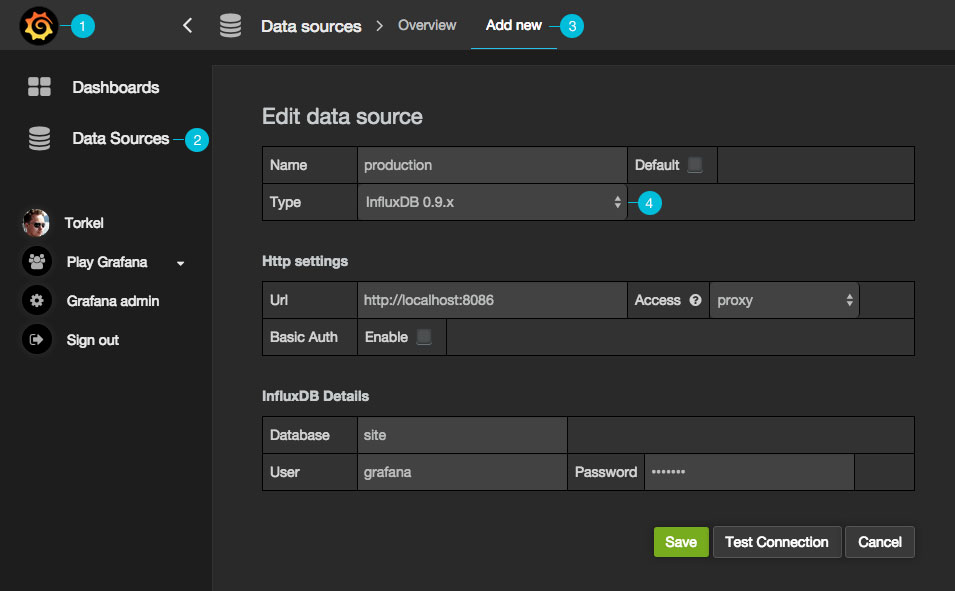
\includegraphics[width=\linewidth]{src/images/05-capitulo-5/datasource-grafana.jpg}
  \caption{Cómo configurar un \gls{term:datasource} para tomar datos de \gls{term:influx}}
  \label{fig:datasource-grafana}
\end{figure}

En la \autoref{fig:datasource-grafana} se pueden ver los pasos para crear un
\gls{term:datasource} en el cliente \eng{web} de \gls{term:grafana}. A
continuación la explicación:

\begin{enumerate}
  \item Abrir el menú haciendo click en el ícono de \gls{term:grafana} en el
  navegador ubicado en la parte superior de la página.

  \item Una vez abierto el menú, hacer click en el enlace \texttt{DataSources}.
  \item Hacer click en el botón \texttt{Add new link} en el navegador.
  \item Llenar el formulario con los datos:
    \begin{itemize}
      \item \textbf{Name:}
      El nombre del \gls{term:datasource}.

      \item \textbf{Default:}
      Si este campo es activado, el \gls{term:datasource} será preseleccionado
      para nuevos paneles.

      \item \textbf{Url:}
      El protocolo \gls{acro:http}, \gls{acro:ip} y puerto de la \gls{term:api}
      de \gls{term:influx}

      \item \textbf{Access:}
      Si se selecciona \texttt{Proxy} , se accede a través del \eng{backend} de
      \gls{term:grafana}.
      Si se selecciona \texttt{Direct}, se accede directamente desde el
      navegador.

      \item \textbf{Database:}
      Nombre de la base de datos de \gls{term:influx}

      \item \textbf{User:}
      Nombre del usuario de la base de datos.

      \item \textbf{Password:}
      Contraseña del usuario de la base de datos.

    \end{itemize}
\end{enumerate}

Una vez creado nuestro \gls{term:datasource} podemos comenzar a crear tableros
en \gls{term:grafana}.

Por ejemplo, a partir de los datos almacenados en \gls{term:influx}, podemos
crear gráficos con la intención de que sean útiles a un responsable de
\gls{acro:it} de la aplicación.

Si quisiéramos medir el tiempo de respuesta de la aplicación \gls{term:ror},
podríamos optar por un gráfico de líneas donde el eje horizontal sea la hora, y
el eje vertical sea el tiempo de respuesta. Dicho gráfico podría desglosarse en
tiempo de \eng{renderizado} de las vistas, tiempo de acceso a las bases de
datos, y otros tiempos.

Para poder recrear el gráfico, se podría aprovechar la información enviada desde
la aplicación \gls{term:ror} en la \autoref{configuracion_de_las_aplicaciones},
y realizar varias consultas a la base de datos \gls{term:influx}.

También podríamos crear un tablero donde se visualice la información generada
por \gls{term:cadvisor} que tenga gráficos que nos muestren el uso de
cpu, memoria, red y sistema de archivos por cada \gls{term:contenedor}.

Usando la herramienta visual provista por \gls{term:grafana} es sencillo crear
un tablero con la información mencionada. En la \autoref{fig:grafana_metricas}
se puede visualizar dicho tablero.

\begin{figure}
  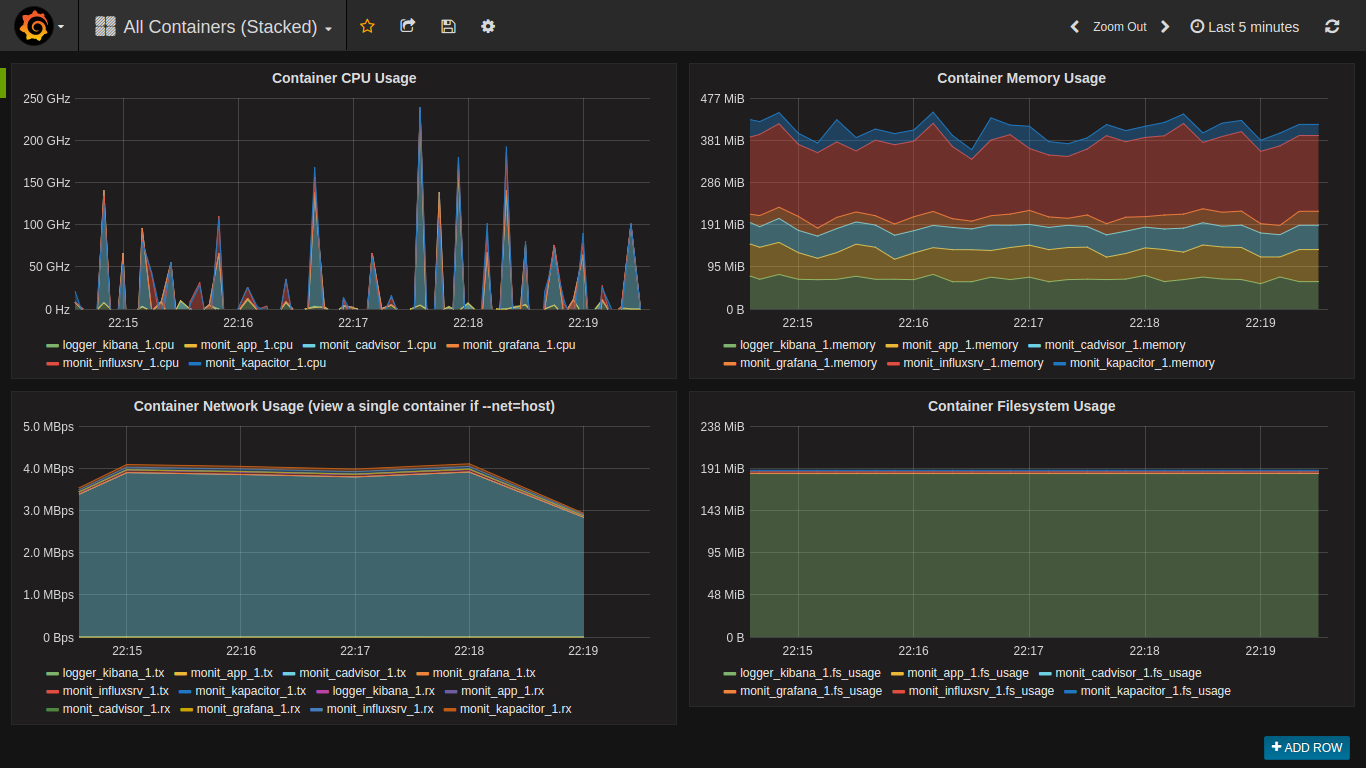
\includegraphics[width=\linewidth]{src/images/05-capitulo-5/grafana_metricas.png}
  \caption{Gráficos generados en \gls{term:grafana} con información de nuestros contenedores}
  \label{fig:grafana_metricas}
\end{figure}

En este capítulo hemos mostrado cómo se pueden configurar algunas herramientas
de visualización para reflejar los datos que hemos almacenado hasta ahora en
\gls{term:influx} y en \gls{term:elasticsearch}. En el capítulo siguiente
mostraremos cómo crear alertas que permitan a los usuarios descubrir de forma
rápida eventos a los que deberían prestar atención.
